\documentclass{article}
\usepackage{../../Self_Style}
\usepackage{../bussproofs}

\EnableBpAbbreviations

\title{Math CS 5 HW 1}
\author{Zih-Yu Hsieh}
\date{\today}

\begin{document}
\maketitle

\begin{ques}\label{q1}
    The following poset is a Heyting algebra: $\{\bot\leq \mu\leq \top\}$. Fill in tables for the Heyting algebra operations.
\end{ques}

\begin{proof}
    Given the basicrules of Heyting algebra (as an easier place of reference for myself):
    \begin{itemize}
        \item $\bot\leq x\leq T$ for all $x\in \mathcal{H}$.
        \item $x\leq y\wedge z$ iff $x\leq y$ and $x\leq z$.
        \item $x\vee y\leq z$ iff $x\leq z$ and $y\leq z$.
        \item $x\leq y\rightarrow z$ iff $x\wedge y\leq z$.
    \end{itemize}
    With these operations in mind, here are the tables for its Heyting Algebra Operations:
    \begin{center}
    \begin{tabular}{ c|c|c|c| } 
        $\wedge$ & $\top$ & $\mu$ &$\bot$\\
        \hline
        $\top$ & $\top$ & $\mu$ & $\bot$ \\ 
        \hline
        $\mu$ & $\mu$ & $\mu$ & $\bot$ \\ 
        \hline
        $\bot$ & $\bot$ & $\bot$ & $\bot$ \\ 
        \hline
    \end{tabular}
    \hfil
    \begin{tabular}{ c|c|c|c| } 
        $\vee$ & $\top$ & $\mu$ &$\bot$\\
        \hline
        $\top$ & $\top$ & $\top$ & $\top$ \\ 
        \hline
        $\mu$ & $\top$ & $\mu$ & $\mu$ \\ 
        \hline
        $\bot$ & $\top$ & $\mu$ & $\bot$ \\ 
        \hline
    \end{tabular}
    \hfil
    \begin{tabular}{ c|c|c|c| } 
        $\rightarrow$ & $\top$ & $\mu$ &$\bot$\\
        \hline
        $\top$ & $\top$ & $\mu$ & $\bot$ \\ 
        \hline
        $\mu$ & $\top$ & $\top$ & $\bot$ \\ 
        \hline
        $\bot$ & $\top$ & $\top$ & $\top$ \\ 
        \hline
    \end{tabular}
    \end{center}
    
\end{proof}

\newpage

\begin{ques}
    A notable absence in our list of logical connectives is negation. Luckily, we can define it in terms of existing connectives: $\neg A:=A \rightarrow \bot$. Let $\mathcal{A}=\{P\}$. The "law of non-contradiction" is the proposition $\neg(P\wedge \neg P)$. A closely related "law" is the "law of excluded middle," which is the proposition $P\vee \neg P$.
    \begin{itemize}
        \item[(a)] Construct a proof tree of $\vdash \neg(P \wedge \neg P)$. (By definition, $(P \wedge (P\rightarrow \bot))\rightarrow \bot$). 
        \item[(b)] Prove that there does not exist a derivation of $\vdash P\vee \neq P$ (Tip: consider the Heyting algebra in the previous problem). 
    \end{itemize}
\end{ques}\label{q2}

\begin{proof}
    
    \hfil

    \begin{itemize}
        \item[(a)] Let $\Gamma=\{P\wedge (P\rightarrow \bot)\}$ as a premise. We get the following proof tree:
        \begin{figure}[h!]
            \centering
            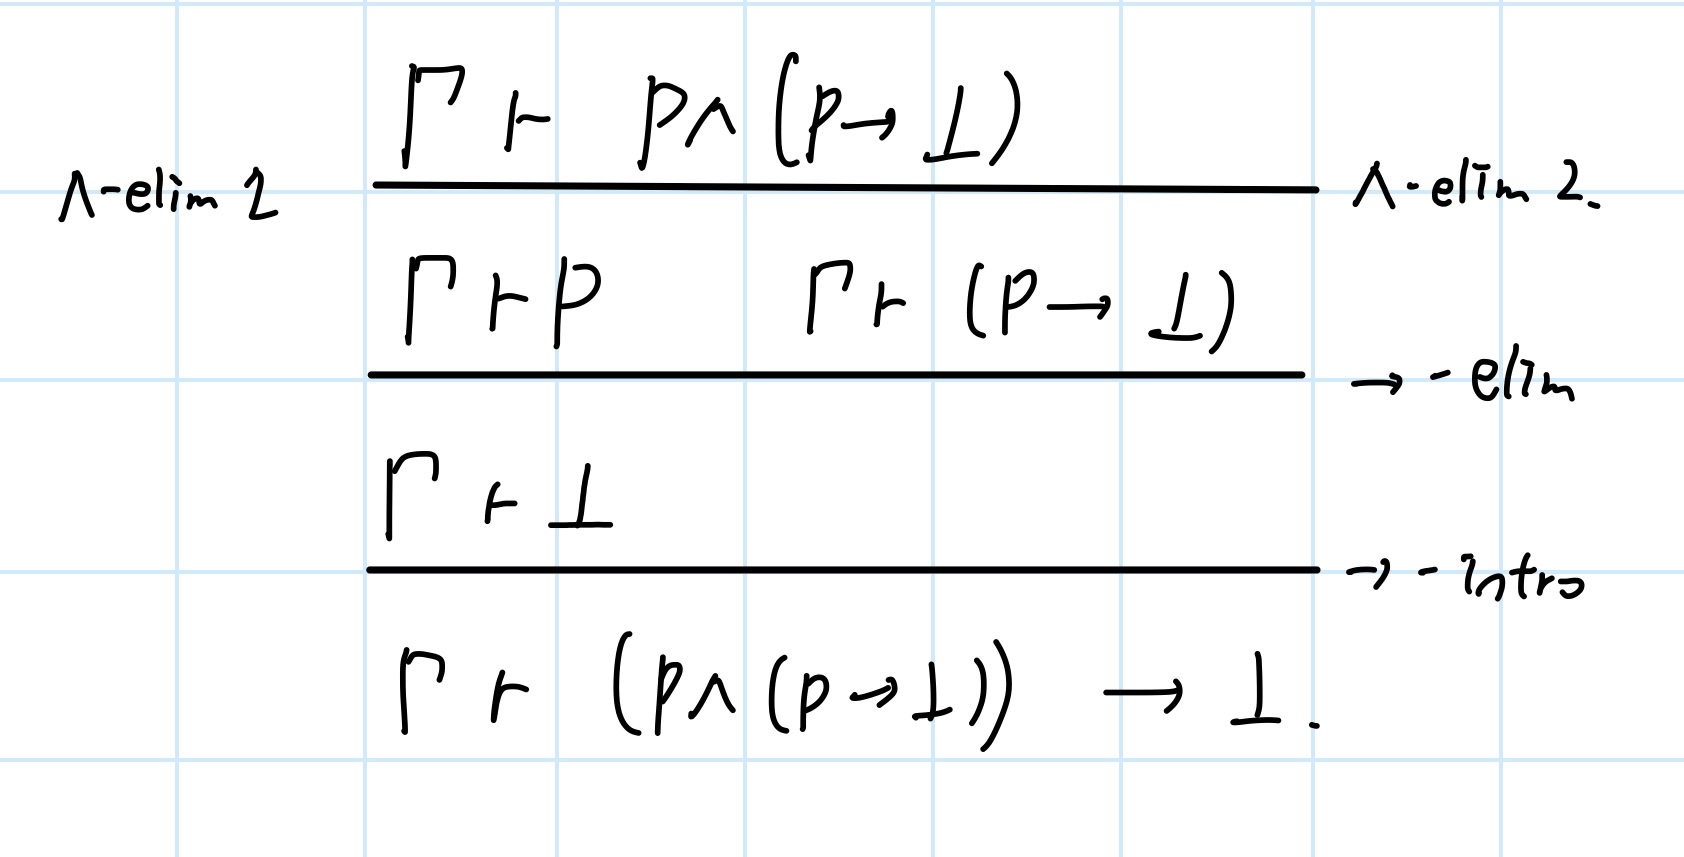
\includegraphics[width=100mm]{2a_proof.jpg}
        \end{figure}

        Where the last $\rightarrow$-intro is also based on the premis (where we form $\Gamma, P\wedge (P\rightarrow \bot)\vdash \bot$).

        (Yeah I failed using the package, I'll try to learn it by the next time).
        \item[(b)] Suppose the contrary that there exists a derivation of $\Gamma\vdash P\vee \neg P$ (given some premise $\Gamma$), if consider the Heyting algebra from the previous problem, define the model $\varphi:\mathcal{A}\rightarrow \mathcal{H}$ by $\varphi(P)=\bot$.  Then, by Soundness Theorem, we derived: 
        $$[\![\Gamma]\!]_\varphi\leq [\![P\vee \neg P]\!]_\varphi = [\![P]\!]_\varphi \vee [\![P\rightarrow\bot]\!]_\varphi = [\![P]\!]_\varphi \vee \left([\![P]\!]_\varphi\rightarrow[\![\bot]\!]_\varphi\right) = \bot \vee (\bot \rightarrow \bot)$$
        Using the previous diagram, we get $[\![\Gamma]\!]_\varphi \leq \bot \vee \bot = \bot$, so $[\![\Gamma]\!]_\varphi = \bot$ based on the inequality. But this becomes an inconsistency (where the premise outputs false). So, this concludes that the derivation of $\Gamma\vdash P\vee \neg P$ doesn't exist.
    \end{itemize}
\end{proof}

\end{document}